\section{The machine-learning pipeline and how it is validated}\label{sec:ml}

The v1 pipeline failed at evaluation, not at fitting. A random split of spatially autocorrelated pixels rewards a model for memorising place, and the score it produced described a task (interpolating inside the same landscape and era) that nobody needs done. Version 2 follows one rule: a headline number is computed under the resampling design that mimics the use it will be put to, against baselines that could embarrass the model, and every fitted quantity, meaning hyper-parameters, feature choices, stacking weights, the applicability threshold and the recalibration constants of Module~B, is fitted inside the training fold only.

\subsection{Three kinds of transfer, six designs}
The framework is used to predict in places it has not seen, in years it has not seen and in climates it has not seen. These are different tasks and no single split covers them; Table~\ref{tab:cv} lists the designs, and the pass criteria are written down now, before any model is fitted. They are defaults to be confirmed at the first gate (\S\ref{sec:plan}), not thresholds tuned to a result.

\begin{table}[t]
\centering
\caption{Validation designs. BSS is the Brier skill score against the stated baseline; the criteria are pre-specified defaults.}\label{tab:cv}
\footnotesize
\begin{tabularx}{\linewidth}{@{}>{\raggedright\arraybackslash\bfseries\sffamily}p{2.55cm}>{\raggedright\arraybackslash}p{4.3cm}>{\raggedright\arraybackslash}p{3.2cm}>{\raggedright\arraybackslash}X@{}}
\toprule
Design & What is held out & Question it answers & Pre-specified criterion\\
\midrule
Spatial-block CV (5 folds, repeated) & Blocks with side $\ge$ residual-variogram range (25~km until estimated), 2~km buffer, folds balanced by event count & New places, same period & BSS vs.\ coordinates-only $\ge0.10$; calibration slope 0.8--1.2\\
Forward chaining & All pixels in years $t{+}1..t{+}3$ after training on years $\le t$ (at least 10 training years) & New years & BSS vs.\ persistence $>0$ at every origin\\
Leave-province-out & One administrative province at a time & Transfer to a management region & BSS $>0$ in the worst province\\
Leave-extreme-year-out & The $k$ driest or hottest years by national SPEI-12 & The years that matter most & Observed event count inside the 90\,\% bootstrap band of predicted\\
Extrapolation CV & Hottest and driest 30\,\% of cells on a CWD--$T_{\max}$ composite; train on the rest & Warmer, drier than seen & Gated hybrid log-loss $\le$ best single component; $\rho_s(\DI,\text{error})\ge0.4$\\
Design-based sample & Independent probability sample of plots (\S\ref{sec:design-based}) & Is the map right, with an honest interval? & Predicted vs.\ observed per class within $\pm0.10$\\
\bottomrule
\end{tabularx}
\end{table}

\textbf{Blocks.} The block side is the practical range of the empirical variogram of residuals from a climate-only model, the distance beyond which residuals are effectively independent \citep{Roberts2017,Valavi2019}. It is then checked with nearest-neighbour distance matching \citep{Mila2022}, which compares the distribution of distances from test to training points in the cross-validation with that from prediction locations to training locations; if the cross-validation is easier than the real task, the blocks are enlarged. Ploton and colleagues showed how badly a random split can overstate large-scale ecological mapping skill \citep{Ploton2020}, and v1's coordinates-only benchmark (Table~\ref{tab:audit}) is the same lesson at small scale. \citet{Meyer2022} add that a map's accuracy statement should travel with the domain in which it was validated, which in this framework is the role of the area of applicability.

\textbf{Nesting.} All tuning runs in an inner loop confined to the outer training blocks. The applicability threshold $\DI^\ast$, the stacking weights and the link-scale recalibration $(a_g,b_g)$ of Module~B are treated as model parameters and are refitted in every outer fold, so that no outer test cell has ever influenced them.

\subsection{Baselines and metrics}
Every design is scored against four baselines: a climatological null (each year's base rate), persistence (the pixel's own event history), a coordinates-only model (a smooth spatial function of position and nothing else) and a replica of the v1 random forest. The coordinates-only benchmark matters most. In the v1 data it explained more variance than the climate deltas did (Table~\ref{tab:audit}); a model that cannot beat a map of its own coordinates has learnt \emph{where}, not \emph{why}.

The hazard model is probabilistic, so it is scored with proper scoring rules. For $N$ person-periods with outcomes $y_j\in\{0,1\}$ and predicted hazards $\hat p_j$, weighted by $1/\pi_0$ for sampled non-events,
\begin{equation}\label{eq:brier}
\mathrm{BS}=\frac1N\sum_{j}(\hat p_j-y_j)^2,\qquad \mathrm{BSS}=1-\frac{\mathrm{BS}}{\mathrm{BS}_{\text{ref}}},\qquad
\mathrm{BS}=\underbrace{\tfrac1N\sum_b n_b(\bar p_b-\bar o_b)^2}_{\text{reliability}}-\underbrace{\tfrac1N\sum_b n_b(\bar o_b-\bar o)^2}_{\text{resolution}}+\underbrace{\bar o(1-\bar o)}_{\text{uncertainty}},
\end{equation}
with the second identity the Murphy decomposition over probability bins $b$. Reliability is the part that matters for decisions, because a hazard that is systematically too high or low changes the ranking of options once it is compounded over 30 years. Calibration is also tested directly by regressing the outcome on the logit of the prediction, $\operatorname{logit}\Prob(y=1\mid\hat p)=a+b\,\operatorname{logit}\hat p$, for which the target is $a=0$, $b=1$; a slope below 1 signals over-fitting, above 1 under-confidence \citep{Steyerberg2010}. The log-loss is the discrete-time likelihood and doubles as the fitting criterion. Because dieback is rare, precision--recall AUC is reported; ROC AUC is reported but never as a headline, since it ignores both calibration and base rate. Expected calibration error is a summary with a known dependence on binning and is never used alone; cumulative-hazard calibration (predicted against observed cumulative incidence by risk decile) is the check that matches the $30$-year use. Overall accuracy and Cohen's $\kappa$ are not used \citep{Pontius2011}. Continuous outputs (attainable height) are scored by the pinball loss of Eq.~\eqref{eq:qr} and by empirical coverage.

\subsection{Prediction intervals, and where they stop being valid}
For attainable height we wrap the quantile models in conformalised quantile regression \citep{Romano2019}: with lower and upper quantile fits $\hat q_{lo},\hat q_{hi}$ and calibration scores $E_i=\max\{\hat q_{lo}(x_i)-y_i,\ y_i-\hat q_{hi}(x_i)\}$, the interval $[\hat q_{lo}(x)-\hat Q,\ \hat q_{hi}(x)+\hat Q]$ with $\hat Q$ the $\lceil(1-\alpha)(n+1)\rceil/n$ empirical quantile of $E_i$ has marginal coverage $\ge1-\alpha$ under exchangeability \citep{Angelopoulos2023}. Under covariate shift the scores can be re-weighted by the density ratio between target and calibration covariates \citep{Tibshirani2019}, but the ratio is undefined where the calibration data have no mass. That is precisely the extrapolation regime, so we do not claim coverage there; intervals outside the area of applicability are drawn hatched, and their empirical coverage is measured in the extrapolation CV and reported.

Applicability is validated as well as used. If the dissimilarity index is informative, prediction error should grow with it; we report skill stratified by $\DI/\DI^\ast$ in the extrapolation CV, and the gate of Eq.~\eqref{eq:gate} is admissible only if the rank correlation between $\DI$ and absolute error is at least 0.4. The decay constant $\kappa=2$ is a default checked against $\kappa\in\{1,2,4\}$ on the same held-out tail.

\subsection{Why in-range validation cannot rank extrapolators: a controlled experiment}
Everything above measures skill on data that resemble the training data. The limits of that are easiest to see in a world where the truth is known. We built two synthetic worlds from the engine of Module~B in which mortality hazard depends on hot-spell temperature and a soil-water index. Training data cover $T_{\max}=24$--34\,$^\circ$C only. The worlds differ in a single trait, the temperature $T_p$ at which residual conductance steepens (38\,$^\circ$C in world A, 47\,$^\circ$C in B), so the data inside the training range are practically indistinguishable, while the hazard beyond it is not (Fig.~\ref{fig:extrap}a,b). Four learners are fitted to the same data: a random forest, the cloglog GLM, the mechanistic model alone (deliberately mis-specified by $+2$\,$^\circ$C in $T_p$, with wider trait spreads and 15\,\% higher capacitance) and the AOA-gated hybrid.

\begin{figure}[t]
\centering
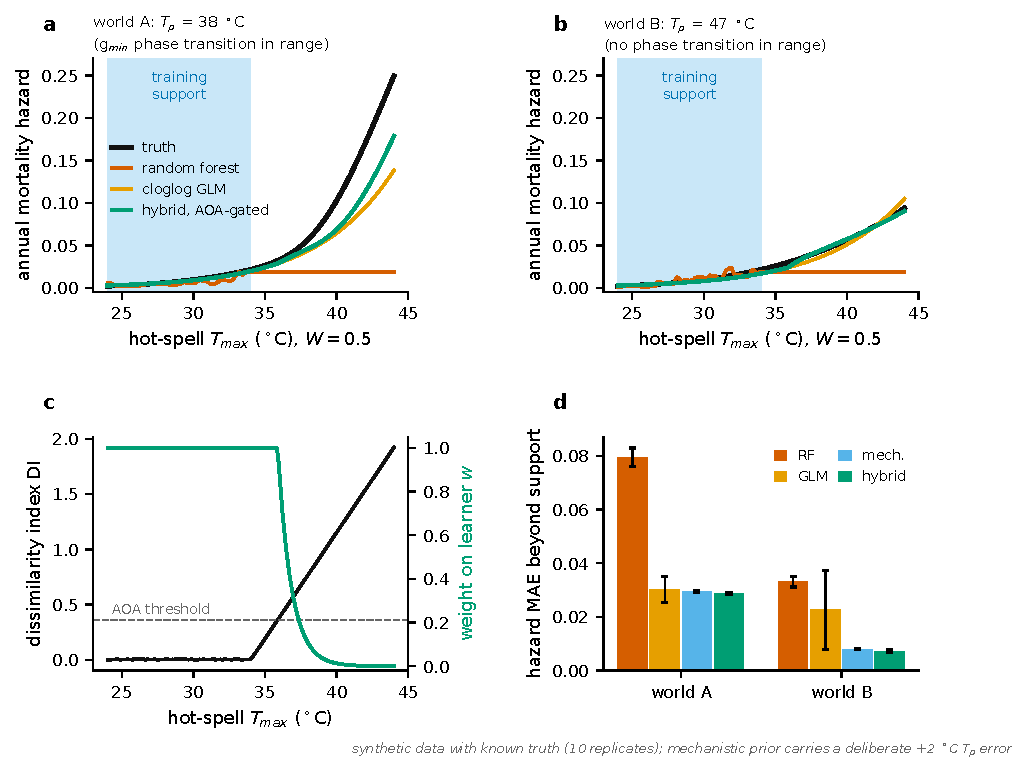
\includegraphics[width=\linewidth]{fig4_extrapolation.pdf}
\caption{Controlled extrapolation experiment on synthetic data with known truth (10 replicates). (a,b)~True hazard and model predictions at fixed soil-water index; the shaded band is the training support. (c)~Dissimilarity index and gate weight $w$ along the temperature axis; the gate hands over to the mechanistic model as the index passes its threshold. (d)~Mean absolute hazard error beyond the training support (mean $\pm$ s.d. of replicates). Illustrative: it demonstrates a mechanism, not the size of the effect in Armenia.}\label{fig:extrap}
\end{figure}

Inside the training range all four methods err by 0.001--0.003 in absolute hazard and cannot be ranked. Beyond it the mean absolute error is, for world A (true mean hazard 0.101), 0.080 for the random forest, 0.030 for the GLM, 0.029 for the mechanistic model and 0.029 for the hybrid; for world B (true mean 0.054), 0.033, 0.023, 0.008 and 0.007. The random forest is worst in both because it holds its last in-range value, as v1's did. The GLM's linear extrapolation on the link scale is an assumption: in B it follows the truth in the typical replicate but its error varies widely (standard deviation 0.015 across replicates), and in A it misses the phase transition. The mechanistic and hybrid models have the lowest error in both worlds, in A only marginally below the GLM, and the hybrid cures nothing: in world A it still under-predicts because its prior places $T_p$ too high, so the transition arrives late. What the design achieves is narrower, and we think more defensible. Extrapolation is made by a model whose form is physically motivated rather than by an accident of the learner; the switch to it is governed by a documented, testable criterion (Fig.~\ref{fig:extrap}c); and its remaining error is bounded by the error of the mechanistic prior, which Module~B's calibration and sensitivity experiments are built to expose.

\subsection{Independent, design-based validation of the products}\label{sec:design-based}
Cross-validation estimates how a modelling procedure performs on new data; it does not estimate the accuracy of the final map, and with clustered or purposive reference data it can mislead in either direction \citep{Wadoux2021}. The claims that will be made to foresters and funders are claims about maps, so they are backed by an independent probability sample whose inference needs no model of spatial structure \citep{Olofsson2014,Stehman2019}. Strata $h$ are cross-classifications of predicted-$V$ class, area-of-applicability status and elevation zone, with stratum weights $W_h$ from mapped areas. The stratified estimator of a proportion (a dieback frequency, or a survival-and-height frequency) and its variance are
\begin{equation}\label{eq:strat}
\hat p=\sum_h W_h\,\bar y_h,\qquad \widehat{\mathrm{Var}}(\hat p)=\sum_h W_h^2\,\frac{s_h^2}{n_h},\qquad n\approx\Big(\frac{\sum_h W_h S_h}{S(\hat p)}\Big)^{2},\quad S_h=\sqrt{p_h(1-p_h)},
\end{equation}
where $S(\hat p)$ is the target standard error and the last expression is the sample size for that target given anticipated stratum proportions $p_h$. For four strata with $W=(0.4,0.3,0.2,0.1)$ and $p=(0.05,0.20,0.50,0.80)$, $\sum_hW_hS_h=0.347$, and a standard error of 0.02 requires $n\approx300$ plots, against about 480 under simple random sampling; this is the origin of the 300-plot minimum in \S\ref{sec:data}. Allocation is proportional to $W_hS_h$ with a floor of 25 plots per stratum and deliberate over-sampling of strata outside the area of applicability. The plots are fixed before any model is fitted, are excluded from training together with a buffer, and accuracy is reported separately inside and outside the area of applicability.

There is one thing no design can do: validate a projection against observations that do not yet exist. What is validated is the machinery that produces projections, in hindcast, in transfer and in extrapolation, and every projected map is accordingly published with its extrapolation footprint instead of an accuracy figure it cannot have.
